%----------------------------------------------------------------------------
\chapter{Implementation} \label{chapter_implementation}
%----------------------------------------------------------------------------
In this chapter, the implementation details of the action language are discussed. It consists of two parts: in Section \ref{section_imp_tech} the tools and frameworks are presented, the new module builds upon. In Section \ref{section_imp_gamma} the integration into the Gamma Framework is discussed, from two different aspects: how the language is integrated into the framework, and how the transformation of the language elements is integrated into the other transformations of the framework. 

%----------------------------------------------------------------------------
\section{Technologies} \label{section_imp_tech}
%----------------------------------------------------------------------------
The applied technologies during the development of the action language correspond to the technologies applied during the development of the Gamma Framework. These are mostly open-source technologies: the target environment is the Eclipse platform, with the Eclipse Modeling Framework (EMF) providing the metamodel specification environment. The Xtext framework was used for the development of the modeling language. The majority of the model transformations was implemented using the Xtend programming language. The complete list can be found in \cite{BenceDipterv}, here only the action language-relevant technologies are presented. 
%----------------------------------------------------------------------------
\subsection{Eclipse Environment}
%----------------------------------------------------------------------------
Eclipse is a popular, open-source integrated development environment (IDE). It is mainly used for Java-related application development, but also supports several other programming languages. It consists of a base workspace and an extensible plug-in system. Using this plug-in system, the develpment environment is easily customizable for different purposes, such as programming in different programming lanugages, modeling (using the Gamma Framework or Yakindu), or testing.

\textbf{Eclipse Modeling Framework:}
The Eclipse Modeling Framework is an Eclipse-based modeling framework and code generation facility. It defines its own structured data model -- called Ecore -- for describing models and providing runtime support for the models. Models are defined using the XML Metadata Interchange (XMI) format, which is supported by various Eclipse plugins developed specifically for this purpose, as EMF is fully integrated into the Eclipse platform. It provides an environment to numerous technologies, including server solutions, persistence frameworks, UI and transformation frameworks.

%----------------------------------------------------------------------------
\subsection{Xtext Framework}
%----------------------------------------------------------------------------
Xtext is an open-source framework for developing (mostly) domain-specific languages (DSLs). It has its own syntax for the definition of textual languages, resembling a context-free grammar extended with mappings to the in-memory representations. Unlike standard parser generators, it generates not only a parser, but also the abstract syntax tree (AST) of the grammar, and also support several other features, such as validation rules and editing support. This is because Xtext is based on the EMF project -- the metamodels of the defined languages are Ecore models --, and it is integrated into the Eclipse environment.

\textbf{Xtend}
Xtend is a general-purpose, high-level programming language based on Java. It is statically typed, object-oriented and uses the type system of Java. Xtend programs are compiled to Java code, thus allowing seamless integration with existing Java libraries. It provides numerous convenient extensions to Java, such as dispatch methods, type inference, operator overloading and extension methods.

%----------------------------------------------------------------------------
\section{Gamma Integration} \label{section_imp_gamma}
%----------------------------------------------------------------------------
Most of the elements of the action language described in Chapter \ref{chapter_theoreticalResults} are already integrated into the Gamma Framework. This integration is twofold: the high-level action language itself -- implemented using the Xtext framework -- had to be integrated into the statechart language, and the the transformation of the statechart models had to be extended with the transformations of the new elements.
%----------------------------------------------------------------------------
\subsection{Integration of the High-level Action Language}
%----------------------------------------------------------------------------
In the Gamma Framework, the statechart language consisted of two parts: the expression language (previously known as constraint language), which also contained the type language, and the statechart language, which contained the elements of statecharts. These statechart elements depended on elements of the expression language. The integration at this level was simple, as only a new element -- the action language -- had to be inserted into the dependency chain. It might be worth to note that these parts each consisted of two eclipse plugins: one for the Ecore metamodel and one for the Xtext grammar and the related functionalities. The resulting plugin dependencies can be seen on Figure \ref{fig:gammaPackage}.

\begin{figure}[H]
	\centering
	\includegraphics[width=70mm, keepaspectratio]{figures/gammaPackage.png}
	\caption{Dependencies of the high-level statechart plugins}
	\label{fig:gammaPackage}
\end{figure}

%----------------------------------------------------------------------------
\subsection{Integration of the Transformations}
%----------------------------------------------------------------------------
For the integration of the action language into the transformations, the existing transformation plugins had to be extended. Even though there were no separate plugins for the transformation of different parts of the statecharts, the dependencies of the classes inside the transformation plugins resembled those of the high-level plugins, thus they were easy to extend. The high-level schematic description of the implementation of the model transformations can be seen on Figure \ref{fig:gammaTransformationComponent}.

\begin{figure}[H]
	\centering
	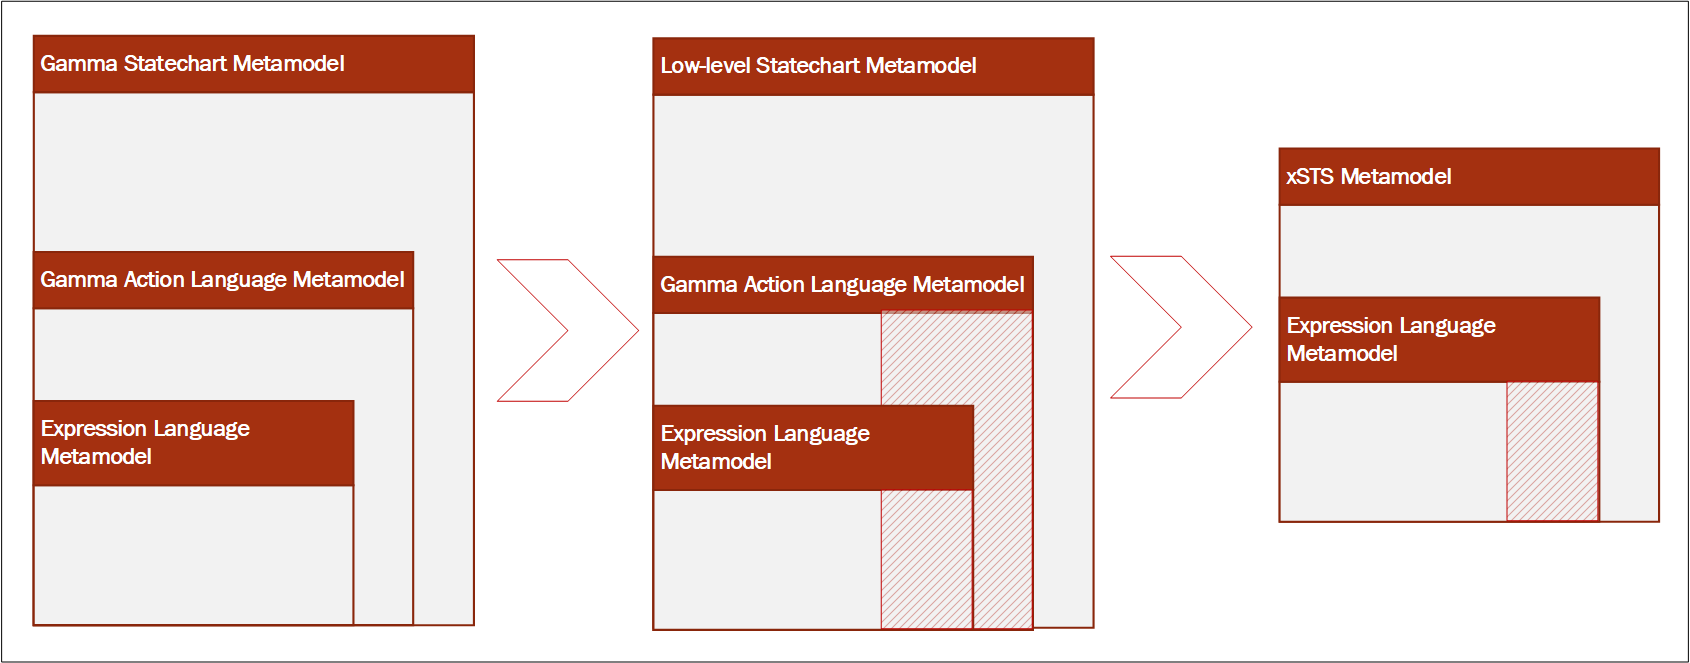
\includegraphics[width=150mm, keepaspectratio]{figures/GammaTransformationComponent.png}
	\caption{Dependencies of the high-level statechart plugins}
	\label{fig:gammaTransformationComponent}
\end{figure}

\textbf{The transformation of access expressions:}

Access expressions -- although not directly part of the action language, but through the expression language -- can only be resolved using actions, due to the current capabilities of the rest of the framework. This resolution happens in the high-level-to-low-level transformation. This means, that access expressions can only be permitted in places where actions can be used too. For this reason, access expressions cannot be used in e.g. initializer expressions of various value declarations. Also, as the resolution of access expressions requires the use of actions, these additional actions must be inserted at the place where these expressions are used. The resolution of the individual access expressions depends on their concrete type.
\begin{itemize}
	\item record access expressions can be resolved relatively easily. As records group individual variables (called fields) under a common name, with the fields also having names, the corresponding variable can be found using these informations, which are explicitly defined at compile time.  
	\item array access expressions impose a great overhead on the system. As the index can be given using any kind of integer-type expression, the current means for the resolution of array access expressions is declaring a temporary variable which is assigned in an if statement that contains a branch for every possible value this index can take.
	\item select expressions are resolved similarly to array access expressions, with the choice being made in a choice statement, with branches guarded by true expressions, thus completely non-deterministically.
	\item function access expressions are resolved as described in Sections \ref{section_tr_elements} and \ref{section_tr_lowlevel} -- by inlining the accessed procedure (as lambdas are not yet supported).
\end{itemize} 
